%# -*- coding:utf-8 -*-
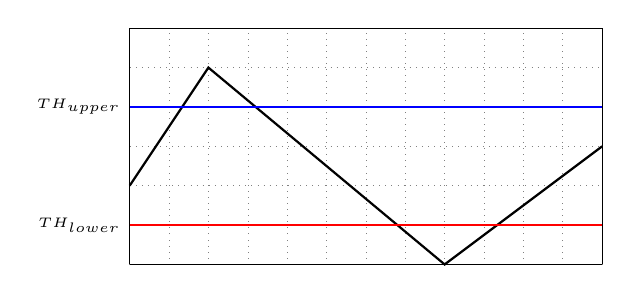
\begin{tikzpicture}[xscale=1.0,yscale=1.0]
\draw [help lines,dotted,step=.5] (0,0) grid (6,3);
\draw [thin] (0,0) -- (0,3);
\draw [thin] (0,3) -- (6,3);
\draw [thin] (0,0) -- (6,0);
\draw [thin] (6,0) -- (6,3);

\draw [thick] (0,1) -- (1,2.5) -- (4,0) -- (6,1.5);
\draw [thick,blue] (0,2) -- (6,2);
\draw [thick,red]  (0,0.5) -- (6,0.5);
% \node [below] at (2,0) {\tiny\textit{lower}};
% \node [below] at (4,0) {\tiny\textit{upper}};
\node [left] at (0,2) {\tiny$\text{TH}_{\text{upper}}$};
\node [left] at (0,0.5) {\tiny$\text{TH}_{\text{lower}}$};
% \draw [thick,red] (0,0.5) -- (2,0.5) -- (2,2.5) -- (4,2.5) -- (4,0.5) -- (6,0.5);
\end{tikzpicture} 